\chapter{Herramientas utilizadas}

En este capítulo se va a hacer una descripción de cada una de las herramientas utilizadas en el proyecto, haciendo especial mención a Net2Plan, que es una herramienta cuya funcionalidad es la de emular y planificar una red de telecomunicación. Dicha herramienta constituye la base para el desarrollo de este proyecto, más concretamente de la prueba de concepto.

Además de Net2Plan, se han utilizado otras herramientas para complementar la funcionalidad de Net2Plan y proveerle diferentes funcionalidad enmarcadas en las tecnologías SDN y NFV. Dichas herramientas son Mininet, para emular redes de telecomunicación; ONOS, un controlador SDN; ETSI-OSM, un gestor y orquestador NFV; y OpenStack, una herramienta para emular una infraestructura IT.

Todas estas herramientas operan en sintonía para llevar a cabo una prueba de concepto exitosa.


\section{Net2Plan}
\label{sec:net2plan}

Net2Plan\cite{net2planbib} es una herramienta \textit{open-source} programada en Java dedicada a la planificación, optimización y simulación de redes de comunicaciones desarrollada por el grupo de investigación GIRTEL de la Universidad Politécnica de Cartagena. En sus inicios, fue concebida como una herramienta para docencia sobre redes de comunicaciones. Sin embargo, actualmente se ha convertido en una poderosa herramienta de optimización y planificación de redes, con un repositorio de recursos para la planificación de redes, tanto para el entorno académico como para el entorno de la industria y la empresa.

Net2Plan está basado en una representación de redes con componentes abstractos, tales como nodos, enlaces, demandas o rutas, entre otros. Esto está pensado para poder planificar cualquier tipo de red, sin importar la tecnología que utilice. Para poder personalizar las redes a gusto del usuario, cada componentes permite añadir atributos. Además, hay clases que permiten modelar una tecnología en concreto (redes IP, WDM o escenarios de NFV).

Una ventaja de esta herramienta es que tiene dos modos de uso: mediante interfaz gráfica (GUI) y línea de comandos (CLI). La interfaz gráfica está pensada para utilizar en sesiones de laboratorio como un recurso formativo, o para poder ver más detalladamente la red sobre la que se está trabajando. Por otro lado, el modo línea de comandos facilita los estudios de investigación, ya que permite automatizar ejecuciones de algoritmos o simulaciones mediante scripts. Como se ha hablado antes, ambos modos permiten utilizar Net2Plan en el entorno académico (investigación o enseñanza) y en el entorno de la industria y la empresa.

\begin{figure}[ht!]
	\centering
	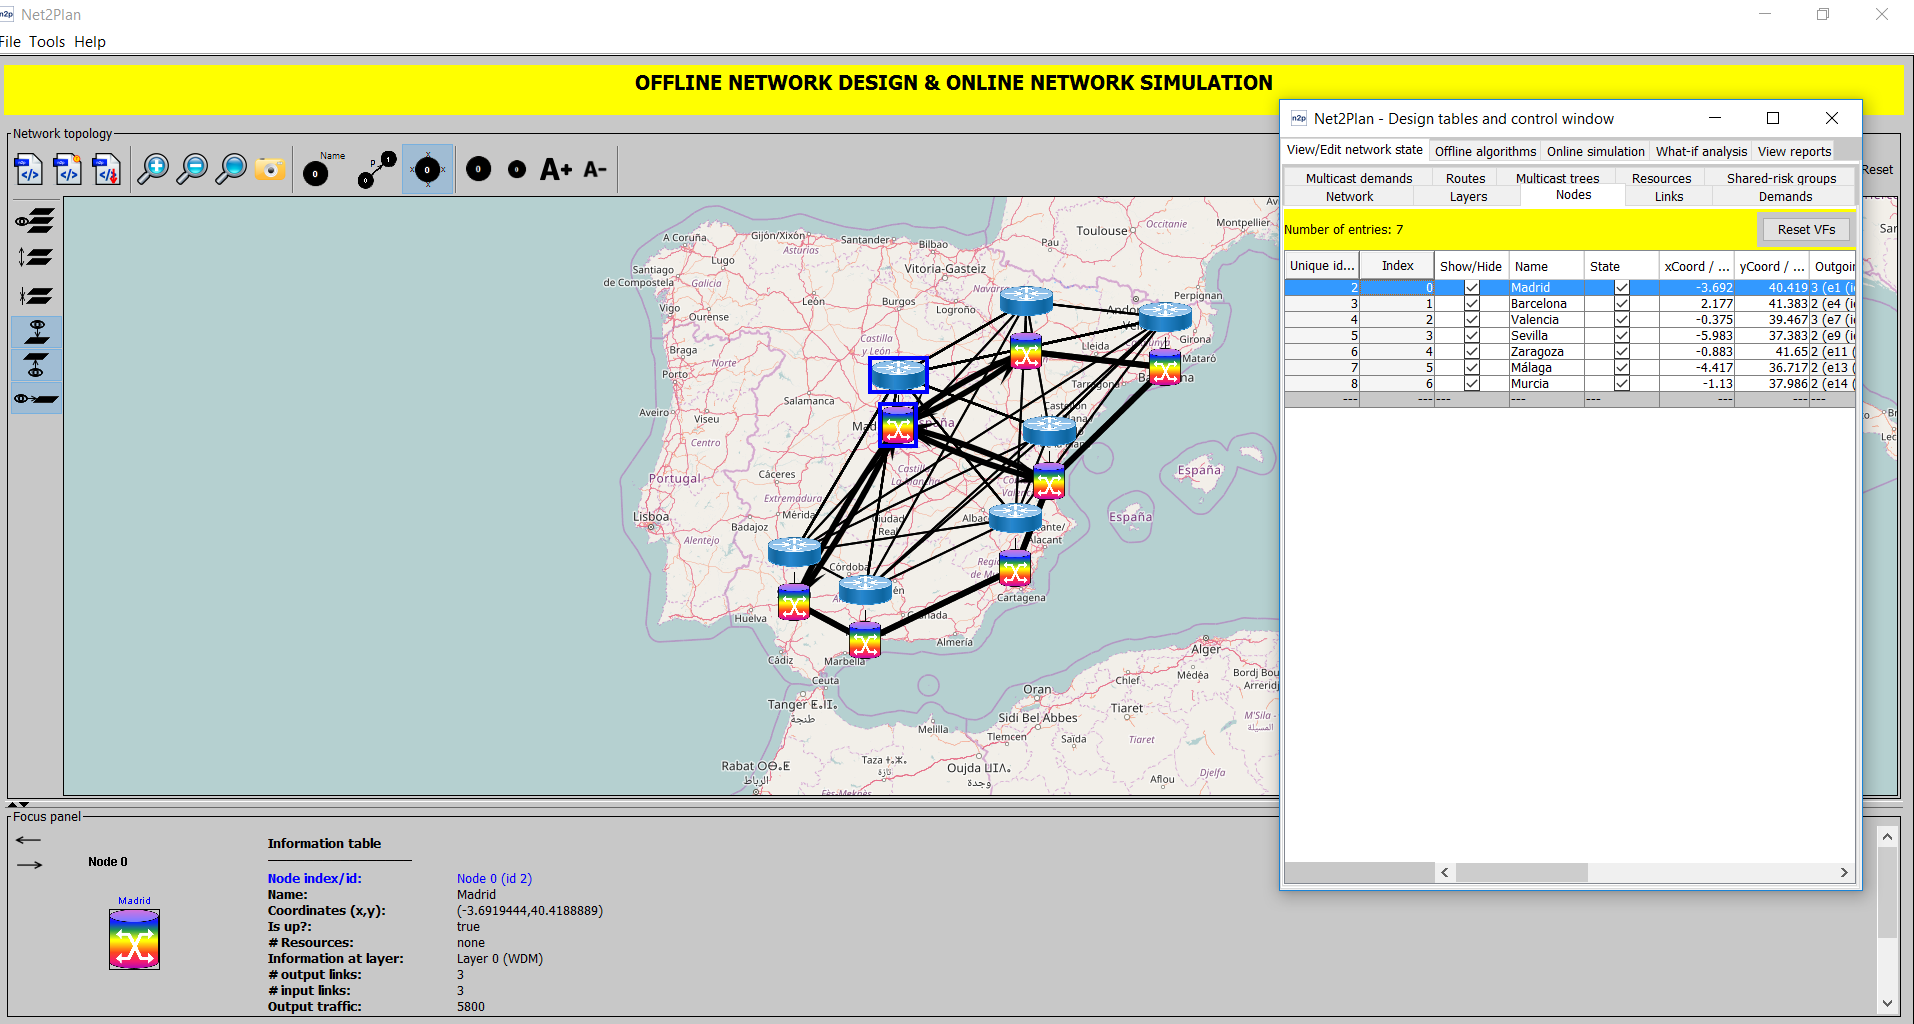
\includegraphics[width=1\linewidth]{imagenes/n2p_redes}
	\caption{Ventana \textit{Offline network desing and online network simulation}}
	\label{fig:n2p_redes}
\end{figure}

En la figura \ref{fig:n2p_redes} se puede ver el aspecto de la interfaz gráfica de Net2Plan, donde se muestra una topología de España con sus respectivas tablas que aportan información detallada de cada uno de los componentes.

\section{Mininet}
\label{sec:mininet}

Mininet\cite{mininetbib} es una herramienta programada en Python cuyo objetivo es el de emular redes de telecomunicación. Permite crear redes con \textit{hosts}, \textit{switches}, controladores y enlaces a un alto nivel. Los \textit{hosts} de Mininet corren bajo un sistema operativo Linux, mientras que los \textit{switches} soportan el protocolo OpenFlow (ver \ref{subsec:openflow}) para mayor flexibilidad respecto a la configuración del \textit{routing} y para integrarlos dentro de un escenario SDN (ver \ref{sec:sdn}).

Mininet tiene una gran polivalencia, y eso permite que sea utilizado en diferentes tareas, tales como investigación, desarrollo, aprendizaje o testeo. Gracias a ello, se puede conseguir emular una red con un comportamiento similar a una real.

Sus principales características son:
\begin{itemize}
	\item Provee un amplio banco de pruebas para desarrollar aplicaciones basadas en OpenFlow.
	\item Permite que varios desarrolladores trabajen de forma concurrente sobre la misma topología de red.
	\item Permite realizar tests exhaustivos de topologías sin necesidad de tener una real.
	\item Incluye una Interfaz de Línea de Comandos que es independiente de la topología emulada y del protocolo que ésta utilice.
	\item Permite crear desde topologías mas sencillas con un único comando hasta topologías realmente complejas haciendo uso de una API programada en Python para definir los componentes con total detalle.
\end{itemize}

Las redes emuladas por Mininet ejecutan aplicaciones estandarizadas de Linux, como el kernel del propio sistema Linux. Esto permite que cualquier desarrollo llevado a cabo y testeado en Mininet pueda ser movido a un sistema real realizando las mínimas modificaciones posibles.

\section{ONOS}
\label{sec:onos}

ONOS (\textit{Open Network Operative System})\cite{onosbib} es un proyecto Open-Source perteneciente a The Linux Foundation. Su principal objetivo es el de crear un controlador SDN para proveedores de servicios de comunicaciones.

Sus principales características son:
\begin{itemize}
	\item \textbf{Escalabilidad:} Ofrece replicación ilimitada mediante virtualización para poder añadir y quitar capacidad al plano de control según sea necesario.
	\item \textbf{Resiliencia:} Provee la disponibilidad requerida por los operadores de red en momentos críticos.
	\item \textbf{Retrocompatibilidad:} Permite añadir o configurar dispositivos y servicios con configuración basada en modelos.
	\item \textbf{Soporte a dispositivos de nueva generación:} Ofrece control en \textit{real-time} para dispositivos OpenFlow.
	\item \textbf{Modularidad:} Las funcionalidades de ONOS están definidas en modulos localizados, lo que hace más fácil probar y mantener el software en buen estado.
\end{itemize}


ONOS está programado en Java y opera como un clúster de nodos idénticos en cuanto al software. Trabaja con modelos y protocolos estandarizados, tales como OpenFlow (ver \ref{subsec:openflow}), NETCONF, OpenConfig, OpenROADM, entre otros.

\clearpage


\begin{figure}[!ht]
	\centering
	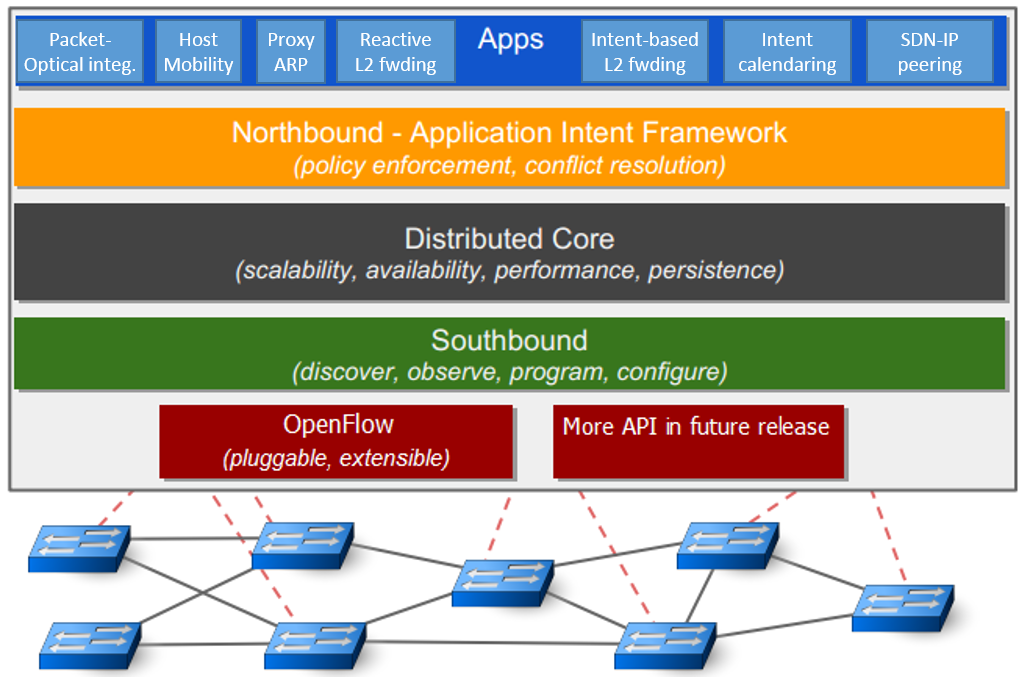
\includegraphics[width=0.7\linewidth]{imagenes/onos_architecture}
	\caption{Arquitectura de ONOS. 
		Fuente: \cite{onostutbib}}
	\label{fig:onosarch}
\end{figure}

En la figura \ref{fig:onosarch} se observa la arquitectura interna de ONOS. En el \textit{Core} se encuentran los controladores de los diferentes servicios que ofrece (TopologyService, DeviceService, HostService, ...), cada uno de ellos destinado a controlar un tipo de componente.

También se puede observar que, para acceder a estos controladores, las aplicaciones necesitan hacer uso de la interfaz \textit{NorthBound}, que se compone de varias subinterfaces que exportan diferentes APIs, como una API REST o una TAPI (\textit{Transport API}).

Por otro lado, para que los controladores puedan tener constancia de los dispositivos de la red, la interfaz \textit{SouthBound} incluye diferentes \textit{drivers}, genéricos o particulares, para poder comunicarse con dispositivos mediante numerosos protocolos estandarizados, como se explicó anteriormente.

\begin{figure}[!ht]
	\centering
	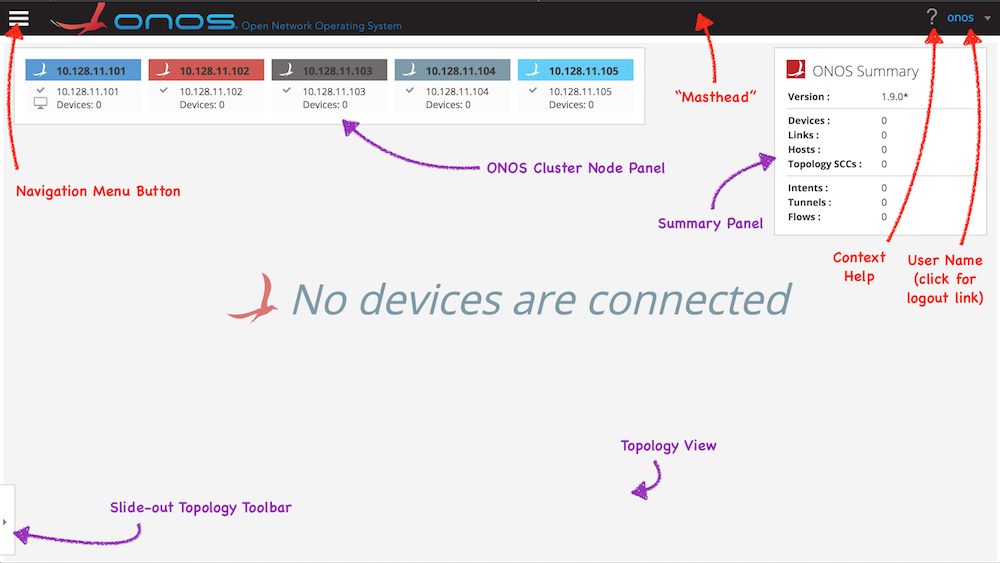
\includegraphics[width=0.8\linewidth]{imagenes/onos_gui}
	\caption{Interfaz Gráfica de ONOS. 
		Fuente: \cite{wikionosbib}}
	\label{fig:onosgui}
\end{figure}

Para facilitar la interacción con el usuario, ONOS ofrece una GUI, como se puede ver en la figura \ref{fig:onosgui}, para ver en más detalle la topología que esta siendo gestionada, así como datos más específicos de cada uno de los dispositivos de la red. 


\subsection{OpenAPI y Swagger}
\label{subsec:openapi}

OpenAPI\cite{openapibib} es una iniciativa creada por varios expertos de la industria y la investigación para estandarizar las descripciones de las RestAPIs. Su principal objetivo es crear y promover un formato de descripción genérico.

Swagger\cite{swaggerbib} es un conjunto de herramientas open-source para definir y documentar REST APIs.

Mediante la colaboración entre OpenAPI, que establece un modelo de APIs común, y Swagger, que permite diseñar una REST API de forma simple, las aplicaciones podrán conectarse entre sí de forma sencilla, y ayudará a tener un mundo más comunicado.

\section{OSM}
\label{sec:osm}

OSM (\textit{Open Source MANO})\cite{osmbib} es un software \textit{open-source} cuya función principal es la orquestación de servicios de red avanzados en infraestructuras NFV heterogéneas. Surge como iniciativa de la ETSI para crear una arquitectura NFV común para los operadores de red.

OSM trabaja con una serie de componentes/elementos que ayudan a definir su arquitectura:

\begin{itemize}
	\item \textbf{VDU (Virtual Deployment Unit):} Es el componente más básico de la arquitectura OSM. Se encarga de definir una máquina virtual. 
	
	\item \textbf{VLD (Virtual Link Descriptor):} Define las conexiones directas entre diferentes componentes de la arquitectura. Hay principalmente dos tipos de VLD: VDU-VDU y VNF-VNF.
	
	\item \textbf{VNFD (Virtual Network Function Descriptor):} Se encarga de definir los recursos necesarios para instanciar un VNF. Incluye diferentes componentes: lista de VDUs que lo definen, lista de VLDs, entre otros.
	
	\item \textbf{NSD (Network Service Descriptor):} Este componente se encarga de definir la configuración de un NS. Incluye diferentes componentes: lista de VNFDs que lo componen, lista de VLDs, parámetros de configuración iniciales, entre otros.
	
	\item \textbf{VNF (Virtual Network Function):} Es el componente que define una función de red virtualizada. Puede estar compuesto de un único VDU o por más de uno.
	
	\item \textbf{NS (Network Service):} Se compone de uno o más VNFs que realizan una función de red más avanzada conjuntamente.
	
	\item \textbf{VIM (Virtual Infrastructure Manager):} Este elemento define un controlador de una o más infraestructuras donde se alojaran las diferentes máquinas virtuales. Es el encargado de comunicar a OSM con las diferentes infraestructuras NFV.
\end{itemize}

\clearpage

\begin{figure}[!ht]
	\centering
	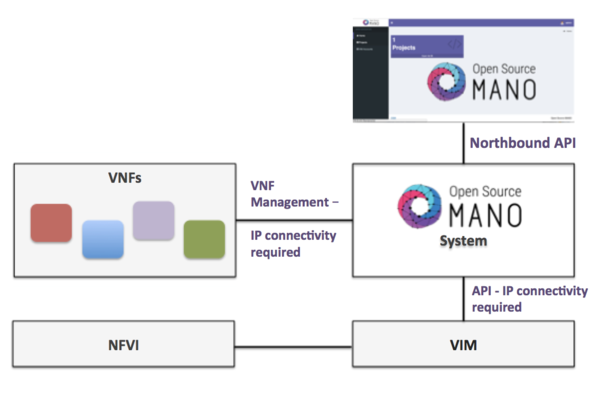
\includegraphics[width=0.8\linewidth]{imagenes/osm_arch}
	\caption{Arquitectura de OSM. 
		Fuente: \cite{osmwikibib}}
	\label{fig:osmarch}
\end{figure}

Para ayudar a explicar el funcionamiento de OSM, la figura \ref{fig:osmarch} da una visión general de la interaccion entre OSM y los diferentes componentes:

\begin{itemize}
	\item \textbf{Interfaz \textit{NorthBound}:} OSM exporta una RestAPI gracias a su interfaz \textit{NorthBound}. Mediante llamadas HTTP (GET, POST, DELETE), el usuario es capaz de ejecutar órdenes en OSM, tales como crear un nuevo VIM o instanciar un nuevo VNF, entre otras.
	
	Para ello, es necesario tener un cliente desde el cuál enviar órdenes. La ETSI ofrece una interfaz gráfica web que se instala al mismo tiempo que OSM y un cliente por línea de comando escrito en Python (ver \ref{subsec:osmclientpython}).
	
	\item \textbf{Conexión con VIM:} OSM permite la comunicación con múltiples tipos de VIM (OpenStack, OpenVIM, VMWare y Amazon Web Services). Para ello, es necesaria conectividad IP entre OSM y el propio VIM, ya que las órdenes enviadas por OSM al VIM para realizar operaciones son hechas mediante una RestAPI.
	
	\item \textbf{Conexión VIM-NFVI:} NFVI (NFV Infrastructure) es el conjunto de recursos (RAM, CPU, HD, entre otros) que son utilizados para instanciar las diferentes máquinas virtuales. El VIM actúa como un controlador de las diferentes NFVIs y gestiona las interacciones entre OSM y ellas.
	
	En estructuras de trabajo pequeñas, es habitual que un VIM y su NFVI estén en la misma máquina física, aunque para estructuras reales de trabajo, la NFVI de un VIM puede estar distribuida en diferentes máquinas físicas, e incluso tener más de una infraestructura.
	
	\item \textbf{VNF \textit{Management}:} cuando un VIM instancia un nuevo VNF, se le asigna una dirección IP para poder acceder a la propia máquina virtual y gestionarla. Por ello, es necesario que haya conectividad IP entre OSM y todos los VNFs. 
\end{itemize}

\subsection{OSMClient}
\label{subsec:osmclientpython}

\section{OpenStack}
\label{sec:openstack}

OpenStack\cite{openstackbib} es un proyecto que sigue el paradigma \textbf{Cloud Computing} para proporcionar un \textit{datacenter} para controlar y gestionar grandes cantidades de recursos de computación, almacenamiento y red. Para facilitar la gestión de recursos, OpenStack provee al usuario una interfaz gráfica a la vez que también exporta una RestAPI para permitir conectividad con aplicaciones externas.

\begin{figure}[!ht]
	\centering
	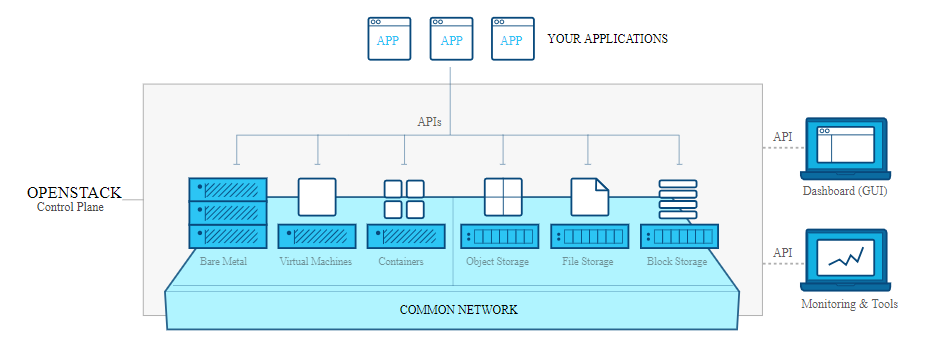
\includegraphics[width=0.9\linewidth]{imagenes/openstack_arch}
	\caption{Arquitectura de OpenStack. Fuente:\cite{openstackbib}}
	\label{fig:openstackarch}
\end{figure}

Está compuesto de diferentes servicios o bloques, encargándose cada uno de ellos de una funcionalidad concreta dentro de la arquitectura. La principal característica de estos servicios es que son accesibles de forma independiente sin dependen los unos de los otros. Los servicios principales de OpenStack son los siguientes:

\begin{itemize}
	\item \textbf{Keystone:}  Este servicio controla la identificación de los diferentes usuarios que se conecten a la infraestructura de OpenStack, y el acceso a según que aplicaciones de los mismos.
	
	\item \textbf{Horizon:} Este servicio es el encargado de mostrar la gestión completa de OpenStack mediante una interfaz gráfica. Desde ella se puede observar con todo detalle que está sucediendo en el sistema y poder gestionar los posibles fallos.
	
	\item \textbf{Nova:} Este servicio está considerado el motor de OpenStack. Es el encargado de desplegar y administrar las diferentes máquinas virtuales instanciadas y otros servicios que se necesiten.
	
	\item \textbf{Neutron:} Este servicio es el encargado de que cada componente desplegado en OpenStack se comunique con los demas y estén interrelacionados.
	
	\item \textbf{Glance:} Este servicio se encarga de gestionar las diferentes imágenes que se usan en la infraestructura.
	
	\item \textbf{Cinder:} Este servicio se centra en el almacenamiento. Facilita el acceso al contenido alojado en las unidades de disco que se encuentren en la infraestructura.
	
	\item \textbf{Swift:} Este servicio es el encargado de almacenar los diferentes archivos del sistema, asegurar su integridad y replicarlos por los diferentes discos de la infraestructura, para hacer más dinámicas la accesibilidad y la disponibilidad.
\end{itemize}

\subsection{OpenStack4Java}
\label{subsec:openstack4j}

OpenStack4Java\cite{openstack4jbib} es una librería REST \textit{open-source} programada en Java para controlar y gestionar un sistema basado en OpenStack.

Permite al usuario realizar una gestión de OpenStack eficiente gracias a sus múltiples módulos, cada uno de ellos focalizado en gestionar un servicio concreto de OpenStack:

\begin{itemize}
	\item \textbf{Identity:} Este módulo se encarga de gestionar el servicio \textbf{Keystone}. Su principal objetivo es el de gestionar el directorio de usuarios, grupos, regiones, servicios y \textbf{endpoints}. Así mismo, se encarga de autenticar y autorizar a los diferentes usuarios para utilizar los diferentes servicios.
	
	\item \textbf{Compute:} Este módulo se encarga de gestionar el servicio \textbf{Nova}. Es el encargado de gestionar las diferentes máquinas virtuales que están corriendo en OpenStack.
	
	\item \textbf{Network:} Este módulo se encarga de gestionar el servicio \textbf{Neutron}. Provee conectividad entre diferentes componentes de OpenStack. Permite a los usuarios crear sus propias redes y añadirles interfaces.
	
	\item \textbf{Image:} Este módulo se encarga de gestionar el servicio \textbf{Glance}. Su principal funcionalidad es la de proveer diferentes servicios para la gestión de imágenes. Permite almacenar imágenes personalizadas por el usuario para inicializar máquinas rápidamente.
	
	\item \textbf{Block Storage:} Este módulo se encarga de gestionar el servicio \textbf{Cinder}. Permite al usuario crear y montar volúmenes para escalar el almacenamiento.
	
	\item \textbf{Object Storage:} Este módulo se encarga de gestionar el servicios \textbf{Swift}. Es el encargado de crear almacenamiento persistente para los diferentes archivos alojados en el sistema.
\end{itemize}


\begin{figure}[!ht]
	\centering
	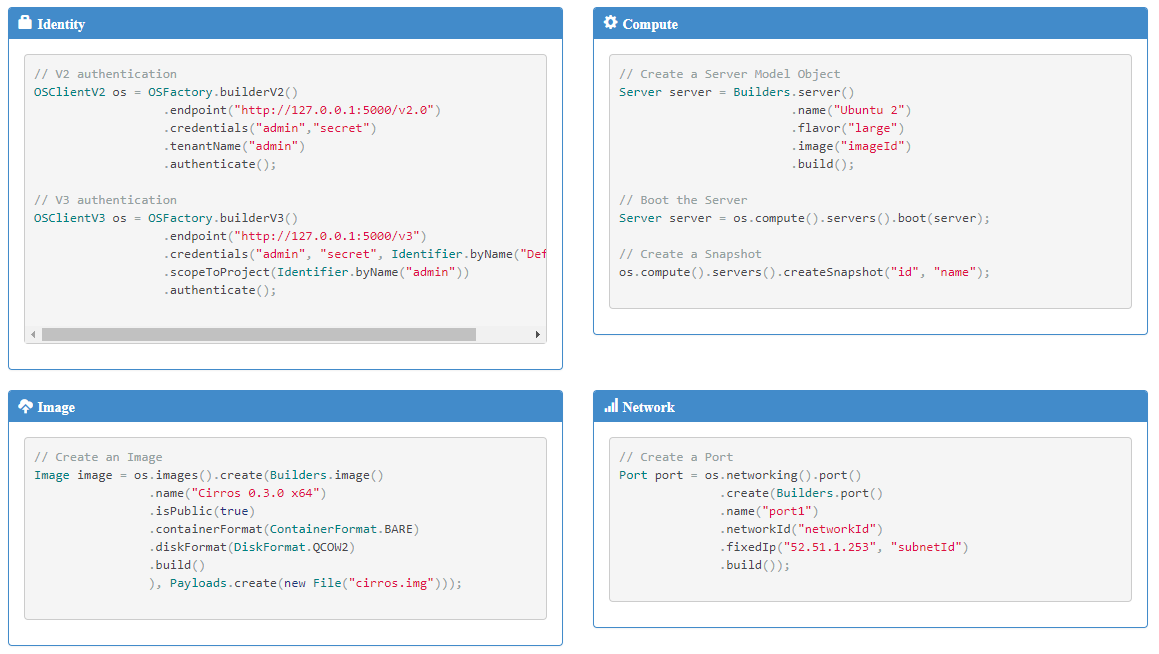
\includegraphics[width=0.8\linewidth]{imagenes/ejemplo_os4j}
	\caption{Ejemplo de uso de OpenStack4j. Fuente:\cite{openstack4jbib}}
	\label{fig:ejemploos4j}
\end{figure}

En la figura \ref{fig:ejemploos4j} se puede ver un breve ejemplo de como utilizar los servicios Identity, Compute, Image y Network.




\cleardoublepage
